\section{Design and Implementation}
\label{sec:implement}

\NM{} is designed as a drop-in replacement for the default memory allocator. It intercepts all memory allocation/deallocation invocations via the preloading mechanism. Therefore, there is no need to change the source code of applications, and there is no need to use custom OS or hardware. Multiple components that differentiate it from existing allocators are further discussed in the remainder of this section.

%\NA{} aims to reduce remote accesses, and balance the workload among different hardware nodes. It also utilizes huge page support to improve the performance, and designs an interleaved heap to accommodate shared objects. 
 
  
%\NA{} also borrows many known mechanisms of existing allocators. First, it utilizes the size class to manage objects. Instead of allocating the exact size, \NA{} will round the size of an allocation to its closest size class. Similar to TcMalloc~\cite{tcmalloc}, \NA{} also utilizes fine-grained size classes for small objects, such as 16 bytes apart for objects less than 128 bytes, and 32 bytes apart for objects between 128 bytes and 256 bytes, then power-of-2 sizes afterwards. Second, it utilizes the ``\textbf{Bi}g-\textbf{B}ag-\textbf{o}f-\textbf{P}ages'' mechanism that all objects in the same bag will have the same size class, and separates the metadata from actual objects. \NA{} only tracks the size information of each page, which helps reduce its memory overhead for the metadata. Third, \NA{} utilizes freelist to manage freed objects. Every freed object will be added into a corresponding freelist, and objects in the freelist will be allocated first in order to reduce possible cache misses. Further, \NA{} utilizes the first word of freed objects to link different objects, which is similar to Linux and TcMalloc~\cite{tcmalloc}. This mechanism helps to reduce the memory overhead, but is prone to memory vulnerabilities, such as buffer overflows and double-frees~\cite{DieHarder, Guarder}.     

\begin{figure*}[h]
\begin{center}
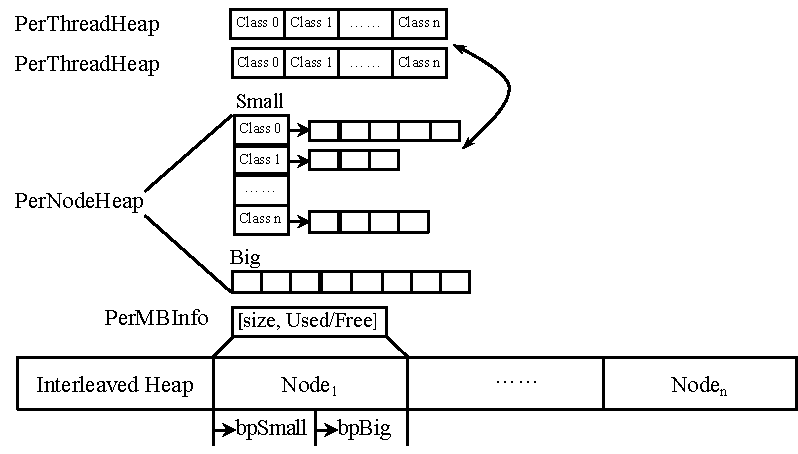
\includegraphics[width=0.8\textwidth]{figure/heaplayout}
%\includegraphics{figure/overview2}
\end{center}
\vspace{-0.1in}
\caption{Overview of \NA{}'s Heap Layout.
\label{fig:overview}}
\vspace{-0.1in}
\end{figure*}

\subsection{Binding-Based Memory Management} 
\label{sec:taskassign}

Existing allocators typically do not schedule threads explicitly, but relying on the default OS scheduler. The OS scheduler performs very well for the UMA architecture that the latency of accessing the memory controller is the same for every core. However, the NUMA architecture imposes additional challenges~\cite{Majo:2015:LPC:2688500.2688509}. If a thread is migrated to a new node, it can break the locality guarantee. It has to access its own stack remotely and reload all data that is already in cache lines of the old node, resulting in a higher memory latency. Also, it may complicate the memory management of objects in its per-thread cache, as further explained in Section~\ref{sec:intro}. 

Due to the importance of avoiding cross-node migration, \NA{} embeds a topology-aware task assignment that also considers load balance.
To balance the workload of each node, \NA{} utilizes a round-robin manner to assign the tasks to different nodes. Basically, a newly-created thread will be assigned to a node that is different from its predecessor. This binding policy ensures that each processor/node will have a similar number of threads, and therefore a similar workload. An alternative approach is to assign the same number of threads as cores to one node, and then assign subsequent threads to the next node. However, this policy has two issues. First, it may cause significant performance issue for applications with the pipeline model due to remote accesses, if threads of different stages are assigned to different memory nodes. Second, it may not fully utilize all memory controllers, if the number of threads is less than the number of cores in total.   In the implementation, \NA{} recognizes the hardware topology via the \texttt{numa\_node\_to\_cpus} API, which tells the relationship between each CPU core and each memory node. It intercepts all thread creations in order to bind a newly-created thread to a specific node. \NA{} employs \texttt{pthread\_attr\_setaffinity\_np} to set the attributes of a thread, and passes the attribute to its thread creation function. Therefore, every thread is scheduled to the specified node upon the creation time. Note that a thread is pinned to a node in \NM{}, instead of a core, which still allows the OS scheduler to perform the load balance when necessarily. 

Based on its thread assignment, \NA{} designs a node-aware memory management. Since a user-space memory allocator only deals with virtual memory, but not physical memory, \textit{\NA{} binds a range of virtual memory to a particular node via the \texttt{mbind} system call}. As shown in Fig.\ref{fig:overview}, each node is mapped to four terabytes (TB) initially, and the interleaved heap is placed in a separate place (Section~\ref{sec:mainthread}).  Therefore, \NA{} is able to compute the physical node information based on a virtual address. More specifically, it could divide the offset (from the heap beginning) by the size of each per-node heap to compute its node index. This design takes the advantage of the huge address space of 64-bits machine to achieve the quick lookup.

Each per-node heap is further divided into two parts, one for small objects (managed with the \texttt{bpSmall} bump pointer) and one for big objects (with the \texttt{bpBig} pointer). An object with the size larger than 512 KB will be treated as a big object, and others are small objects. The space for big objects are separated from that for small objects so that we could utilize huge pages for big objects, as discussed in Section~\ref{sec:hugepage}. Another difference between small objects and big objects is that small objects are managed by size classes, while big objects of each node are tracked in a global free list.  For small objects, \NM{} utilizes the ``\textbf{Bi}g-\textbf{B}ag-\textbf{o}f-\textbf{P}ages'' (BiBOP) mechanism that all objects in the same bag will have the same size class, and separates the metadata from actual objects. In order to track the size information of objects, \NM{} utilizes one megabytes (MB) as a basic unit, where the information is tracked in a PerMBInfo data structure (as shown in Fig.~\ref{fig:overview}. A big object in \NM{} is always aligned to megabytes, and small objects in the same MB (called as a bag) will has the same size. For a big object that is larger than 1MB, all corresponding bytes in the PerMBInfo will be set to the specific size upon the allocation. \NM{} embeds the availability information of each chunk to the \texttt{PerMBInfo} structure, using the lowest significant bit of the size. \NM{} is able to coalesce multiple continuous big objects into a bigger object upon deallocations.  

For each size class of small objects, \NM{} maintains a freelist for each node and for each thread. Every size class has 16-byte difference when the size is less than 128 bytes, and then 32 bytes apart for objects less than 256 bytes. When an object is larger than 256 bytes, its size class will be always power of two. Except those ones stated in Section~\ref{sec:mainthread}, \NA{} ensures node-aware memory allocations that an allocation is guaranteed to be allocated from the local node physically. \textit{For each deallocation, \NM{} ensures that an object is always placed into a freelist based on the origin of this object}. More specifically, for small objects, it will be placed into the current thread's freelist \textbf{only if} it is originated from the same node that the current thread belongs to. Otherwise, it will be placed to the per-node freelist of its original owner. A big object is always placed into the freelist of its owner. \textit{\NM{} also handles allocations carefully to ensure the locality}. For small objects, an allocation will be satisfied from the freelist of the current thread, where all freed objets is originated from the local node, if there exists some freed objects. Otherwise, the thread will migrate some freed object from the per-node freelist. If its per-node freelist is empty, then it will get a batch of never-used objects from the bag of a size class. Allocations of big objects is always satisfied from per-node freelist first, before getting a new object from the per-node heap.   


\textit{Cache Warmup Mechanism:} For small objects, \NM{} also borrows the cache warmup mechanism of TcMalloc~\cite{tcmalloc}. TcMalloc utilizes a \texttt{mmap} system call to obtain multiple pages (depending on the class size) from the OS each time, when it is running out of the memory for one size class. For such a memory block, TcMalloc inserts all objects of this block into its central freelist at one time. Since TcMalloc utilizes the first word of each object as the pointer for the freelist, this mechanism warms up the cache by referencing the first word of each object during the insertion. According to our observation, this warmup mechanism improves the performance of one application (\texttt{raytrace}) by 10\%. Based on our understanding, the performance improvement is caused by data prefetches, since inserting objects to the freelist has a simple and predictable pattern. \NM{} employs a similar mechanism for small objects with the size less than 256 bytes, and adds all objects inside a page to the per-thread freelist. 
%A bump pointer is used to track the position of never-used objects, whose updates do not require to be exactly one page each time. By comparison, TcMalloc may waste some memory in the end of each block, if the block size is not equal to multiple times of the class size.   

\subsection{Interleaved Heap} 
\label{sec:mainthread}

\NA{} proposed an interleaved heap for shared objects. Based on our observation, most NUMA performances issues identified by existing NUMA profilers are related to shared objects~\cite{XULIU, MemProf}. These shared objects are typically allocated in the main thread, but are passed to children threads later. Allocating the physical memory for shared objects in one node may introduce load imbalance issue, and therefore causing significant number of remote accesses and potential interconnect congestion. Therefore, \NA{} reserves a range of memory for shared objects, called as ``Interleaved Heap'' in Fig.~\ref{fig:overview}. \NA{} utilizes the \texttt{mbind} system call to specify that  physical pages of this range will be allocated from all nodes interleavedly. This design helps balance the volume of memory accesses of all memory controllers, reducing interconnect congestion and load imbalance. 

\begin{comment}
\begin{wrapfigure}{r}{0.6\textwidth}
\centering
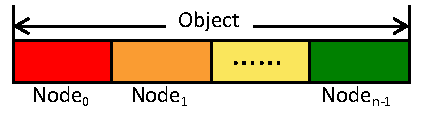
\includegraphics[width=3in]{figure/blockwise}
\vspace{-0.1in}
\caption{Block-wise Memory Allocation\label{fig:blockwise}}
\vspace{-0.1in}
\end{wrapfigure}
\end{comment}
 
During the implementation, \NA{} only allocates potentially-shared objects from the main thread in the interleaved heap. Although it may benefit the performance, if shared objects allocated in children threads are also using the interleaved heap. However, the overhead of tracking shared objects is typically larger than the performance benefit, based on our evaluation (skipped in the paper). 

It is very important to identify shared objects correctly and efficiently. \NA{} utilizes the allocation/deallocation site to identify shared objects: every allocation of the main thread is treated as a shared one initially, and is allocated from the interleaved heap. The callsite-based method is aligned with the intuition, since the shared behavior of a callsite is determined by the program logic. When a newly-allocated object is deallocated before creating children threads, all objects from the corresponding callsite are considered to be private objects, and then are only allocated from the per-node heap afterward. Overall, \NM{} monitors memory allocation/deallocation pattern to identify whether a corresponding callsite is shared or not. 
%Therefore, \NA{} utilizes the callsite to differentiate objects, which is determined by the program logic.  

%However, it is very challenging to determine the allocation callsite \textit{uniquely} and \textit{efficiently} due to multiple reasons. First, function pointers are removed in most applications if they were compiled with an optimization, which makes it impossible to obtain return addresses (and callsite) via built-in functions. Second, applications have a wrapper for memory allocations, which requires multiple levels of call stacks to uniquely identify one callsite. Although there exist mechanisms to encode calling context explicitly~\cite{DBLP:conf/icse/SumnerZWZ10, DBLP:conf/cgo/ZengR0AJ014}, they require the recompilation of the applications. The \texttt{backtrace} function can obtain the callsite, but it is too slow to be used in production environment.
\NM{} requires to track the shared pattern for each callsite. For the performance reason, \NA{} further proposes to utilize the sum of the stack position and the return address of the allocation to identify a callsite, called ``\textit{callsite key}''. 
  When memory allocations are invoked in different functions, their stack positions are likely to be different. The return address (of the application) tells the invocation placement inside the same function. However, this design cannot completely avoid mis-identification issue,  where multiple allocations inside the allocation wrapper will be treated as the same callsite. However, the mis-identification will not cause any correctness issue, but only performance issue. During the implementation, we have thought about two other mechanisms. One is to obtain the callsite correctly with the \texttt{backtrace} function, but it is too slow to be used in production environment. The other mechanism will require the recompilation to encode calling context explicitly~\cite{DBLP:conf/icse/SumnerZWZ10, DBLP:conf/cgo/ZengR0AJ014}.
  
%   A shared callsite can be treated as a private callsite, if an object from  these callsites invokes the deallocation before creating children threads. For the performance reason, \NA{} obtains the return address quickly via a constant offset, where the offset is uniquely determined after the compilation of \NA{}. 

\NA{} utilizes a hash table to track the status of every callsite. Upon every allocation of the main thread, \NA{} checks the status of the allocation callsite, with the callsite key as described above. If the callsite is identified as a shared callsite, the current allocation will be satisfied from the interleaved heap. Otherwise, it will be allocated from the per-node heap. Upon deallocations, \NM{} marks an allocation callsite as private, if an object from this callsite has been deallocated before creating other threads. 

%When an allocation is satisfied in the callsite and the callsite is new, the corresponding allocation will be tracked in the second hash table. The second hash table will be checked upon deallocations, where the corresponding allocation callsite will be marked as private if an object is allocated in the same epoch. 

\subsection{Explicit Huge Page Support} 
\label{sec:hugepage}
%Modern hardware typically installs with huge page support.
\NA{} employs explicit huge page support to further improve the performance. The size of a huge page is 2 megabytes (MB) in the current OS. Based on the existing study~\cite{hugepages}, huge pages can reduce Translation Look-aside Buffer (TLB) misses that may significantly affect the performance, since a huge page covers a larger range of memory than a normal page (4 KB). Reducing TLB misses helps reduce the interferences on the cache utilization caused by TLB misses, and therefore reduces cache misses. Huge pages could also reduces the contention in the OS memory manager, since it imposes less page faults and requires much less time on page table management. We observed around 10\% performance improvement for some applications, when we are using huge page support. 

However, existing studies showed that the transparent huge page support of the OS is not good for the performance~\cite{Gaud:2014:LPM:2643634.2643659, DBLP:conf/asplos/PanwarBG19}. In fact, it may have some harmful impact on the performance of NUMA systems. First, it can cause the \textit{hot page effect} when multiple frequently-accessed objects were  mapped  to  the  same  physical  page, causing the overloading of the corresponding memory node. Second, huge pages are more prone to \textit{page-level false sharing}, when multiple threads are accessing different data inside the same page. Besides that, the huge page may increase the memory footprint~\cite{DBLP:conf/asplos/MaasAIJMR20}, if only a partial range of a huge page is accessed. 

\NA{} utilizes huge pages explicitly to avoid these issues. Ideally, if huge pages are only utilized for private objects, then there will be no hot page effect and page-level false sharing. Also, if huge pages are only utilized for big objects that are larger than the page size, or if all small objects in a huge page will be allocated, then there is no need to worry about the memory consumption. \NA{} takes these consideration into account. \NM{} only employs huge pages for large objects with the size larger than a huge page, and for small objects that are predicted to be used a lot. For the latter one, \NM{} employs the history information to predict, and only uses huge pages for a size class that has allocated at least one bag of objects. 

%In addition to large objects that has the size larger than the size of a huge page, huge pages are only utilized for small objects that are predicted to be used a lot.  \NA{} employs the history of memory allocation to predict this. 
%Each per-node heap is further divided into two parts as illustrated in Fig.~\ref{fig:overview}: small objects will be allocated from the first half and will be allocated using small pages, while big objects will be allocated from the second half with huge pages (2MB). When a big object (with the huge page) is utilized for small objects, only frequently-allocated small objects can utilize such an object. We believe that our design balances the performance and memory consumption.   

\subsection{Efficient Object Migration} 

\label{sec:moveobjects}

\NM{} maintains per-thread heaps and per-node heaps in order to reduce the synchronization overhead. This design also requires to move freed objects between different freelists. 
When a per-thread freelist has too many objects, some of them should be moved to the thread's per-node freelist so that other threads could re-utilize these freed objects, reducing the memory consumption. Similarly, each per-thread list may need to obtain freed objects from its per-node heap, when a thread is running out the memory. Frequent migrations require an efficient mechanism. \NM{} utilizes singly link lists to manage freed objects, imposing an additional challenge of migrating objects efficiently. 

One straightforward method is to traverse the  freelist from the head in order to collect a specified number objects, and then moves them at a time. Actually both TcMalloc and TcMalloc-NUMA utilize such a mechanism, which   actually has multiple issues. First, traversing a list will actually pollute the cache of the current thread unnecessarily, especially when a thread is moving out objects. \NM{} utilizes the first word of each freed object as the pointers for the linked list, where traversing these objects will bring these objects to the cache that the current thread do not need. Second, it may introduce thread contention, when multiple threads are migrating freed objects from the per-node freelist concurrently. We observed  20\% slowdown for some applications, due to this straightforward mechanism. \NM{} further proposes an efficient mechanism to migrate objects efficiently. 

\begin{wrapfigure}{r}{0.6\textwidth}
\centering
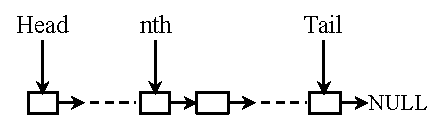
\includegraphics[width=3in]{figure/perthreadlist}
\vspace{-0.1in}
\caption{Avoiding the traverse of per-thread freelist\label{fig:perthreadlist}}
\vspace{-0.1in}
\end{wrapfigure}
In order to avoid the pollution on the per-thread cache, each per-thread freelist maintains two pointers that pointing to the least recent object (shown as the \texttt{Tail} object) and the $nth$ object separately, as shown in Fig.~\ref{fig:perthreadlist}. Maintaining the pointer to the $nth$ object requires only a forward traverse to obtain the pointer of $(n-1)th$ object, and then a thread can migrate $n$ objects (between $(n-1)th$ and the \texttt{Tail} object) easily. 
After the migration,  the \texttt{Tail} pointer can be set to the original $nth$ object. However, this mechanism alone cannot reduce the lock contention when multiple threads are concurrently obtaining objects.

\begin{wrapfigure}{r}{0.6\textwidth}
\centering
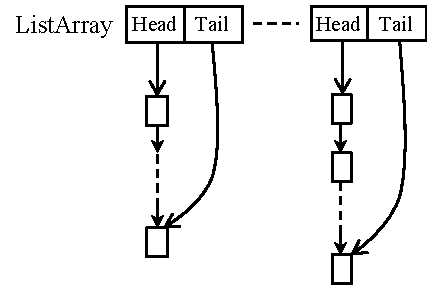
\includegraphics[width=3in]{figure/listarray}
\vspace{-0.1in}
\caption{An array of freelists for per-node heap\label{fig:listarray}}
\vspace{-0.2in}
\end{wrapfigure}
In order to avoid the bottleneck of the per-node heap, \NM{} introduces a circular array of freelists as shown in Fig.~\ref{fig:listarray}, where the number of entries is a variable that can be changed by the compilation flag. Each entry has two pointers, head and tail separately. In order to support the put and get operations to the freelist, this array has two pointers, \texttt{toGetIndex} and  \texttt{toPutIndex}. If a thread tries to obtain freed objects from the per-node heap, it will obtain all  objects pointed by the \texttt{toGetIndex}, and increment the index afterward. If the freelist pointed by the \texttt{toGetIndex} has no freed objects, there is no freed objects in the per-node freelist for this size class.  The put operation will utilize the pointer \texttt{toPutIndex}. There are two scenarios for the put operation. First, a thread may put an freed object directly to the per-node freelist, if this object is originated from a different node that the thread does not belong to. In this case, the object will be placed into the freelist pointed by the \texttt{toPutIndex}, but the index is not updated after the deallocation. Second, when freed objects in a per-thread freelist is above the predefined watermark, the thread will migrate a batch of objects to the freelist pointed by the \texttt{toPutIndex}. After this migration, the current freelist is considered to be full, and will update the index to the next entry in the circular array.

   

%When a thread migrates freed objects to the per-node heap, it will add the list of objects to the freelist pointed by \texttt{toPutIndex}, and update the index after the migration. Similarly, iAs described above, if a thread running on the other node just deallocates an object to the per-node heap, then this object will be added to the head of the freelist pointed by  \texttt{toPutIndex}, but the index is not changed after the deallocation.  
 

\subsection{Other Mechanisms}
\label{sec: others}

\paragraph{Node-Local Metadata:} \NM{} guarantees that all of the metadata is always allocated in the same node, based on its thread binding as described in Section~\ref{sec:taskassign}. Such metadata includes per-node and per-thread freelists for different size classes, and freelists for big objects. Similarly, \NM{} utilizes the \texttt{mbind} system call to bind the memory to a specific node.  

\paragraph{Encouraging Memory Reutilization:} In \NM{}, every thread has its own freelists for each size class so that there is no need to acquire the lock when an allocation can be satisfied from its per-thread heap, similar to TcMalloc. That is, two threads will not share the same per-thread heap. However, some applications may create new threads after some threads have exited. \NM{} re-utilizes the memory for these exited threads. Basically, \NM{} intercepts thread joins and cancels so that it can assign heaps of exited threads for newly-created threads, and re-utilize their heaps correspondingly.  


\paragraph{Transparent Huge Page Support:} During the development, we noticed that excessive memory consumption can be imposed when the OS enables transparent huge pages by default. In order to reduce memory consumption, \NM{} makes multiple threads share the same bag (for the same size class), instead of having a separate bag for each thread. If each thread is running out of the memory, it obtains multiple objects at a time from the corresponding bag. Currently, if a class size is less than one page, then we will at most get objects with the total size of one normal page. Otherwise, it will get 4 objects (with the size less than 64 KB) or 2 objects afterward. Based on our evaluation, this mechanism actually reduces the memory consumption for multiple times for a machine with 128 cores and 8 nodes, with the transparent huge page support by default.  

%we propose the combination of per-node heap and per-thread cache. In order to reduce the contention, \NM{} will obtain multiple objects at a time from the per-node heap. 

 
%https://queue.acm.org/detail.cfm?id=2852078

